%%%%%%%%%%%%%%%%%%%%%%%%%%%%%%%%%%%%%%%%%%%%%%%%%%%
%% LaTeX book template                           %%
%% Author:  Amber Jain (http://amberj.devio.us/) %%
%% License: ISC license                          %%
%%%%%%%%%%%%%%%%%%%%%%%%%%%%%%%%%%%%%%%%%%%%%%%%%%%

\documentclass[a4paper,11pt]{book}
\usepackage[T1]{fontenc}
\usepackage[utf8]{inputenc}
\usepackage{lmodern}
%%%%%%%%%%%%%%%%%%%%%%%%%%%%%%%%%%%%%%%%%%%%%%%%%%%%%%%%%
% Source: http://en.wikibooks.org/wiki/LaTeX/Hyperlinks %
%%%%%%%%%%%%%%%%%%%%%%%%%%%%%%%%%%%%%%%%%%%%%%%%%%%%%%%%%
\usepackage{hyperref}
\usepackage{graphicx}
\usepackage[english]{babel}
\usepackage[a4paper,top=2cm,bottom=2cm,left=2cm,right=2cm]{geometry}
\usepackage{lscape}
\usepackage{caption}
\usepackage{amsmath}
\usepackage{listingsutf8}
\usepackage{listings}
\usepackage{float}
\usepackage{amsmath}
\usepackage{subfig}
\usepackage{xcolor}
\usepackage{textcomp}
\usepackage{wrapfig}
\usepackage{rotating}
\usepackage{epstopdf}
\usepackage{commath}

\definecolor{codegreen}{rgb}{0,0.6,0}
\definecolor{codegray}{rgb}{0.5,0.5,0.5}
\definecolor{codepurple}{rgb}{0.58,0,0.82}
\definecolor{backcolour}{rgb}{0.95,0.95,0.92}

\lstdefinestyle{mystyle}{
	backgroundcolor=\color{backcolour},   
	commentstyle=\color{codegreen},
	keywordstyle=\color{magenta},
	numberstyle=\tiny\color{codegray},
	stringstyle=\color{codepurple},
	basicstyle=\ttfamily\footnotesize,
	language = C++,
	%frameround=fttt,
	%frame = trBL,
	firstnumber = last,
	breakatwhitespace=false,         
	breaklines=true,                 
	captionpos=b,                    
	keepspaces=true,                 
	numbers=left,                    
	numbersep=5pt,                  
	showspaces=false,                
	showstringspaces=false,
	showtabs=false,                  
	tabsize=2
}

\lstset{style=mystyle}

\captionsetup{tableposition=top,figureposition=bottom,font=small}
%%%%%%%%%%%%%%%%%%%%%%%%%%%%%%%%%%%%%%%%%%%%%%%%%%%%%%%%%%%%%%%%%%%%%%%%%%%%%%%%
% 'dedication' environment: To add a dedication paragraph at the start of book %
% Source: http://www.tug.org/pipermail/texhax/2010-June/015184.html            %
%%%%%%%%%%%%%%%%%%%%%%%%%%%%%%%%%%%%%%%%%%%%%%%%%%%%%%%%%%%%%%%%%%%%%%%%%%%%%%%%
\newenvironment{dedication}
{
   \cleardoublepage
   \thispagestyle{empty}
   \vspace*{\stretch{1}}
   \hfill\begin{minipage}[t]{0.66\textwidth}
   \raggedright
}
{
   \end{minipage}
   \vspace*{\stretch{3}}
   \clearpage
}

%%%%%%%%%%%%%%%%%%%%%%%%%%%%%%%%%%%%%%%%%%%%%%%%
% Chapter quote at the start of chapter        %
% Source: http://tex.stackexchange.com/a/53380 %
%%%%%%%%%%%%%%%%%%%%%%%%%%%%%%%%%%%%%%%%%%%%%%%%
\makeatletter
\renewcommand{\@chapapp}{}% Not necessary...
\newenvironment{chapquote}[2][2em]
  {\setlength{\@tempdima}{#1}%
   \def\chapquote@author{#2}%
   \parshape 1 \@tempdima \dimexpr\textwidth-2\@tempdima\relax%
   \itshape}
  {\par\normalfont\hfill--\ \chapquote@author\hspace*{\@tempdima}\par\bigskip}
\makeatother

%%%%%%%%%%%%%%%%%%%%%%%%%%%%%%%%%%%%%%%%%%%%%%%%%%%
% First page of book which contains 'stuff' like: %
%  - Book title, subtitle                         %
%  - Book author name                             %
%%%%%%%%%%%%%%%%%%%%%%%%%%%%%%%%%%%%%%%%%%%%%%%%%%%

% Book's title and subtitle
\title{
	\includegraphics[width=0.7\textwidth]{Immagini/UniBg.png}
	\\ \Huge \textbf{Navigazione basata su inseguimento di frecce} \\ \huge \textit{\textbf{Relazione di progetto}} \\ \bigskip \huge Progetto del corso Robotica (principi e progetto)\\ Università degli Studi di Bergamo \\ \huge A.A. 2019/2020}
% Author
\author{\textsc{Calegari Andrea - 1041183}
		\\ \textsc{Paganessi Andrea - 1040464}
		\\ \textsc{Piffari Michele - 1040658}}

\begin{document}
	
	\frontmatter
	\maketitle
	%%%%%%%%%%%%%%%%%%%%%%%%%%%%%%%%%%%%%%%%%%%%%%%%%%%%%%%%%%%%%%%%%%%%%%%%
	% Auto-generated table of contents, list of figures and list of tables %
	%%%%%%%%%%%%%%%%%%%%%%%%%%%%%%%%%%%%%%%%%%%%%%%%%%%%%%%%%%%%%%%%%%%%%%%%
	\tableofcontents
	\listoffigures
	
	
	
	\mainmatter
	\chapter{Stato dell'arte}
	Obbiettivo: andare a implementare sistema di \textit{visual navigation} per la base robotica in figura ~\ref{fig:BaseRobotica} facendo uso del supporto in figura ~\ref{fig:SupportoRialzato}.

Per il progetto del corso di Robotica è stato implementato un algoritmo in
C++ che, partendo da un’immagine di input, risulta essere in grado di individuare
frecce (sfruttando la libreria OpenCV) composte dalla somma di due differenti forme: un rettangolo, di un certo colore, e un triangolo, di un secondo colore differente
marcatori di un determinato colore di forma circolare , fornendo in output le coordinate dei centri di tali marcatori rispetto ad un sistema di riferimento.
La scelta della forma dei marcatori è ricaduta sulle frecce poichè esse rappresentano \textit{simboli} in grado di fornire una doppia informazione: \textit{direzione e orientamento}, che rappresentano appunto i dati forniti in uscita dalla nostra libreria, la cui struttura a blocchi è rappresentata in figura ~\ref{fig:CodeStructure}.

L’algoritmo è stato sviluppato col presupposto di avere a disposizione un sistema visivo composto da una sola telecamera RGB; inoltre esso fornisce la possibilità di impostare l’angolo che la telecamera forma con l’asse orizzontale e l'altezza della camera stessa rispetto al terreno.


\begin{figure}
	\centering
	\includegraphics[width=\textwidth]{Immagini/CodeStructure.jpeg}
	\caption{Struttura del codice}
	\label{fig:CodeStructure}
\end{figure}

\begin{figure}
	\centering
	\includegraphics[width=0.5\textwidth]{Immagini/BaseRobotica.jpg}
	\caption{Base robotica addetta alla movimentazione}
	\label{fig:BaseRobotica}
\end{figure}

\begin{figure}
	\centering
	\includegraphics[width=0.5\textwidth]{Immagini/SupportoCamera.jpg}
	\caption{Base verticale sulla quale andare ad inserire la camera}
	\label{fig:SupportoRialzato}
\end{figure}
	\chapter{Camera}
	\section{Scelta della camera}
Inizialmente si è scelta come camera \textit{SpotLight Pro Webcam}, una webcam già utilizzata in un progetto precedente \textit{Trust} (fig. ~\ref{fig:TrustCam}).
\begin{figure}[H]
	\centering
	\includegraphics[width=0.3\textwidth]{Immagini/TrustCam.jpg}
	\caption{Camera utilizzata inizialmente}
	\label{fig:TrustCam}
\end{figure}
È stato però notato che, questa camera, non era in grado di dare sufficienti garanzie di funzionamento stabile in alcune delle più comuni condizioni luminose.

Si è deciso quindi di passare ad una camera di tipo industriale, in grado di fornire delle prestazioni più stabili e affidabili. 
La scelta è ricaduta sulla camera della casa produttrice \textit{IDS (Imaging Development System)}: si tratta del modello \textit{UI-1221LE-C-HQ} equipaggiata con la lente \textit{BM2420} della casa \textit{Lensagon}.
\begin{figure}[H]
	\centering
	\includegraphics[width=0.3\textwidth]{Immagini/camera-usb2-ueye-le-rev2-boardlevel-m12-1.jpg}
	\caption{Camera utilizzata successivamente}
	\label{fig:Cam}
\end{figure}

La camera in Fig.\ref{fig:Cam} ha un'otturatore globale che permette di acquisire tutta l'immagine istantaneamente e non in modo progressivo come la camera  \textit{SpotLight Pro Webcam}



\section{Vericale o orizzontale?}
TODO che vuol dire?
\section{Come ottenere le immagini dalla camera?}
Per ottenere le immagini dalla camera è stato necessario iscriversi presso il sito web della casa produttrice e scaricare i driver necessari all'installazione.
La videocamera ha diverse opzioni di acquisizione tra cui anche una grandezza dell'immagine diversa dal classico 480x640 ma per ragioni di semplicità si è scelto di lasciare invariate le impostazioni di default.




	\chapter{Gestione delle maschere}
	\section{HSV}
Nella strutturazione del progetto ci è venuto molto naturale andare a lavorare con una scala di colori HSV. Ma perchè non applicare un filtraggio basato su RGB?
Come noto nella letteratura, nell'ambito dell'\textit{image recognition} è usuale il problema di andare a mascherare un colore piuttosto che un altro, come nel nostro caso.
Potremmo voler trovare, sempre per esempio, oggetti rosso, scannerizzando nell'immagine solamente colori (255,0,0) nella scala RGB; con questo approccio andremmo ad applicare una condizione troppo stringente ai colori.
Si potrebbe pensare, come soluzione a questa condizione parecchio stringente, di trovare colori in un range di rossi, come per esempio {(130,0,0);(255,0,0)}: il problema comunque persisterebbe proprio per il fatto che il rosso è ottenuto come combinazione di più colori primari, e non come un solo singolo colore.
Potremmo pensare dunque, di andare a fondo del problema,cambiando gli intervalli dei valori RGB per tutti i colori primari ma sarebbe uno sforzo non secondario e probabilmente con risultati poco significativi.
È necessario un metodo che abbia meno parametri per semplificare l'identificazione dei colori; questo metodo è rappresentato dall'utilizzo del HSV.


\begin{figure}[H]
	\centering
	\includegraphics[width=0.5\textwidth]{Immagini/HSV_RGB.jpeg}
	\caption{RBG vs HSV}
	\label{fig:HSV}
\end{figure}
Si può notare come, in Fig\ref{fig:HSV}, il colore rosso sia definito in un range ben chiaro di un solo valore(\textit{Hue}) mentre \textit{Saturation }and \textit{Value} servono sono a limitare ulteriormente la gamma di tonalità di rosso accettabili. 
\section{Frecce o cerchi?}
Nel progetto precedentemente svolto, si erano individuati cerchi di diversa grandezza per testare le funzionalità della libreria OpenCV nell' object detection.
Ovviamente l'utilizzo di cerchi limita di molto l'espressività del simbolo in quanto un cerchio non può, per sua natura identificare una direzione, men che meno un verso.
Le frecce sono quindi la soluzione più naturale al problema di identificare con un simbolo una direzione ed un verso che poi un eventuale robot mobile potrà seguire.

TODO mettere foto cerchi e frecce
foto maschera

\section{Maschere}
Le maschere sono fondamentali nel processo di object detection tramite la libreria OpenCV.
Queste ultime sono immagini binarie(bianco e nero) e sono utilizzate da tutte le funzione di identificazione dei contorni e interpolazione di punti presenti in OpenCV.
La seguente linea di codice,

\begin{lstlisting}
	inRange(original_image_hsv, Scalar(MinH_R, MinS_R, MinV_R), Scalar(MaxH_R, MaxS_R, MaxV_R), hsv_red);
\end{lstlisting}

permette di identificare tutti gli oggetti di colore rosso e di salvarli nella Matrice \textit{hsv\_red}.
\section{Erosione e dilatazione}
L'erosione e la dilatazione sono tecniche note allo stato dell'arte attuale utili per rimuovere rumore da una immagine.

\begin{figure}[H]
	\centering
	\includegraphics[width=0.5\textwidth]{Immagini/erosion_dil.png}
	\caption{Erosione e dilatazione}
	\label{fig:erosion_dil}
\end{figure}

Nel caso preso in considerazione da questo report è stato necessario applicare la tecnica di erosione solamente alla parte inferiore dell'immagine in quanto, se applicata nella parte superiore, avrebbe eliminato oltre al rumore anche un'eventuale freccia che sarebbe apparsa molto piccola.
	\chapter{Identificazione delle forme}
	\section{Definizione del problema}
Il capitolo precedente ha mostrato come sia possibile ottenere dei contorni delle figure da un'immagine a colori.
È ora necessario identificare la forma di ciascuno di questi contorni riconoscendo così i vari quadrati e rettangoli presenti nell'immagine che avessero, una volta acquisiti dalla camera, il colore specificato. Come ultimo passaggio va svolto il controllo per verificare che esista o meno una freccia; quest'ultima altro non è che un triangolo e un rettangolo sufficientemente vicini fra di loro.

\section{Interpolazione}
Per approssimare il contorno ottenuto e filtrato attraverso le mask, come spiegato nel Capitolo 3, è necessario usare una funzione che approssima il contorno individuato con un altro poligono avente meno vertici così che la distanza tra di essi sia inferiore ad una certa soglia. Tale funzione è così definita nella libreria OpenCV:

\begin{lstlisting}
	void approxPolyDP(InputArray curve, OutputArray approxCurve, double epsilon, bool closed)
\end{lstlisting}

Si è reso necessario effettuare un tuning del parametro \textsl{epsilon} in quanto, per frecce diverse, a distanza variabile e con orientazione non fissa sono stati individuati differenti valori ottimali. Il valore che più si adattava a tutti i casi presi in considerazione è stato ottenuto sperimentalmente e corrisponde a \textsl{epsilon = 0.045}.

La funzione di cui sopra restituisce quindi una lista di poligoni ognuno dei quali è descritto da una lista di vertici.
Il passo successivo è stato cercare nella lista dei poligoni un elemento che avesse 4 lati nel caso di un rettangolo e 3 in quello di un triangolo:

\begin{lstlisting}
	if(result->total >= 3  && result->total <= 3 && fabs(cvContourArea(result, CV_WHOLE_SEQ))>lower_area_triang)
\end{lstlisting}
\begin{lstlisting}
	if(result->total >= 4  && result->total <= 6 && fabs(cvContourArea(result, CV_WHOLE_SEQ))>lower_area_rect)
\end{lstlisting}

Sempre per via sperimentale è stato possibile scoprire che vincolando il poligono che approssima il quadrilatero cercato ad avere tra i 4 e i 6 lati, la probabilità di riconoscere correttamente un rettangolo aumentava.Per il triangolo questo non si è reso necessario vista la buona probabilità di successo nella ricerca vincolata a 3 lati.

Ottenuti ora tutti i triangoli e i rettangoli sufficientemente grandi nella figura va affrontato il problema del riconoscimento di ogni freccia presente nel seguente modo:
\begin{itemize}
	\item \textbf{} per ciascun rettangolo identificato, si calcola la distanza che intercorre tra esso e ogni triangolo riconosciuto. Per calcolare la distanza tra due figure è necessario:
	\begin{itemize}
		\item \textbf{}definire il centro del rettangolo, tramite funzioni della libreria OpenCV;
		\item \textbf{}ottenere il baricentro del triangolo;
		\item \textbf{}calcolare la distanza cartesiana tra i due punti appena individuati.
	\end{itemize}
	\item \textbf{} si tiene in considerazione solamente la distanza minore calcolata.
	\item \textbf{} si confronta suddetto valore con una soglia sperimentale; se questo valore è minore allora si può assumere che il triangolo e il quadrato presi in considerazione siano una freccia, altrimenti si scarta la coppia.
	\item \textbf{} la freccia appena rilevata viene aggiunta alla lista delle frecce rilevate nell'immagine.
\end{itemize}
Per ogni freccia, che ora altro non è che una coppia di punti,
\begin{equation}
	\begin{split}
		C_{triangolo}=(x_t,y_t)\\ 
		C_{rettangolo}=(x_r,y_r)
	\end{split}
\end{equation}

vanno identificati nell'ordine:
\begin{itemize}
	\item \textbf{}il centro della freccia, ottenuto come il punto medio del segmento che collega i due centri che definivano la freccia precedentemente.
	$$
		C_{freccia}=(\dfrac{x_t+x_r}{2},\dfrac{y_t+y_r}{2})
	$$
	\item \textbf{}L'inclinazione della freccia nel piano, calcolata come:
		\begin{equation}
			\begin{split}
				\phi=atan(\frac{\Delta y}{\Delta x}), dove\\
				\Delta y=y_t-y_r\\
				\Delta x=x_t-x_r
			\end{split}
		\end{equation}
	\item \textbf{}L'area dell'oggetto freccia, ricavata come somma dell'area del triangolo e del quadrato.
	
	
	

\end{itemize}	
	\chapter{Dalle \textit{pixel coordinates} alle \textit{world coordinates}}
	\section{Scelta della camera}
Nel capitolo precedente è stato illustrato un metodo atto all'identificazione delle frecce che rientrano nel campo visivo della camera. Viene ora trattato come sia possibile ottenere la posizione della freccia, precedentemente ottenuta, nelle coordinate 3D XYZ rispetto alla base del robot.



\begin{figure}
	\centering
	\includegraphics[width=0.5\textwidth]{Immagini/TrustCam.jpg}
	\caption{Camera utilizzata inizialmente}
	\label{fig:TrustCam}
\end{figure}


\section{Vericale o orizzontale?}
\section{Come ottenere le immagini dalla camera?}

	\chapter{Matrici di rotazione}
	\begin{figure}[H]
	\centering
	\includegraphics[width=0.8\textwidth]{Immagini/RoboticsFrames-2.jpg}
	\caption{Frames scelti}
	\label{fig:frames}
\end{figure}

\begin{figure}[H]
	\centering
	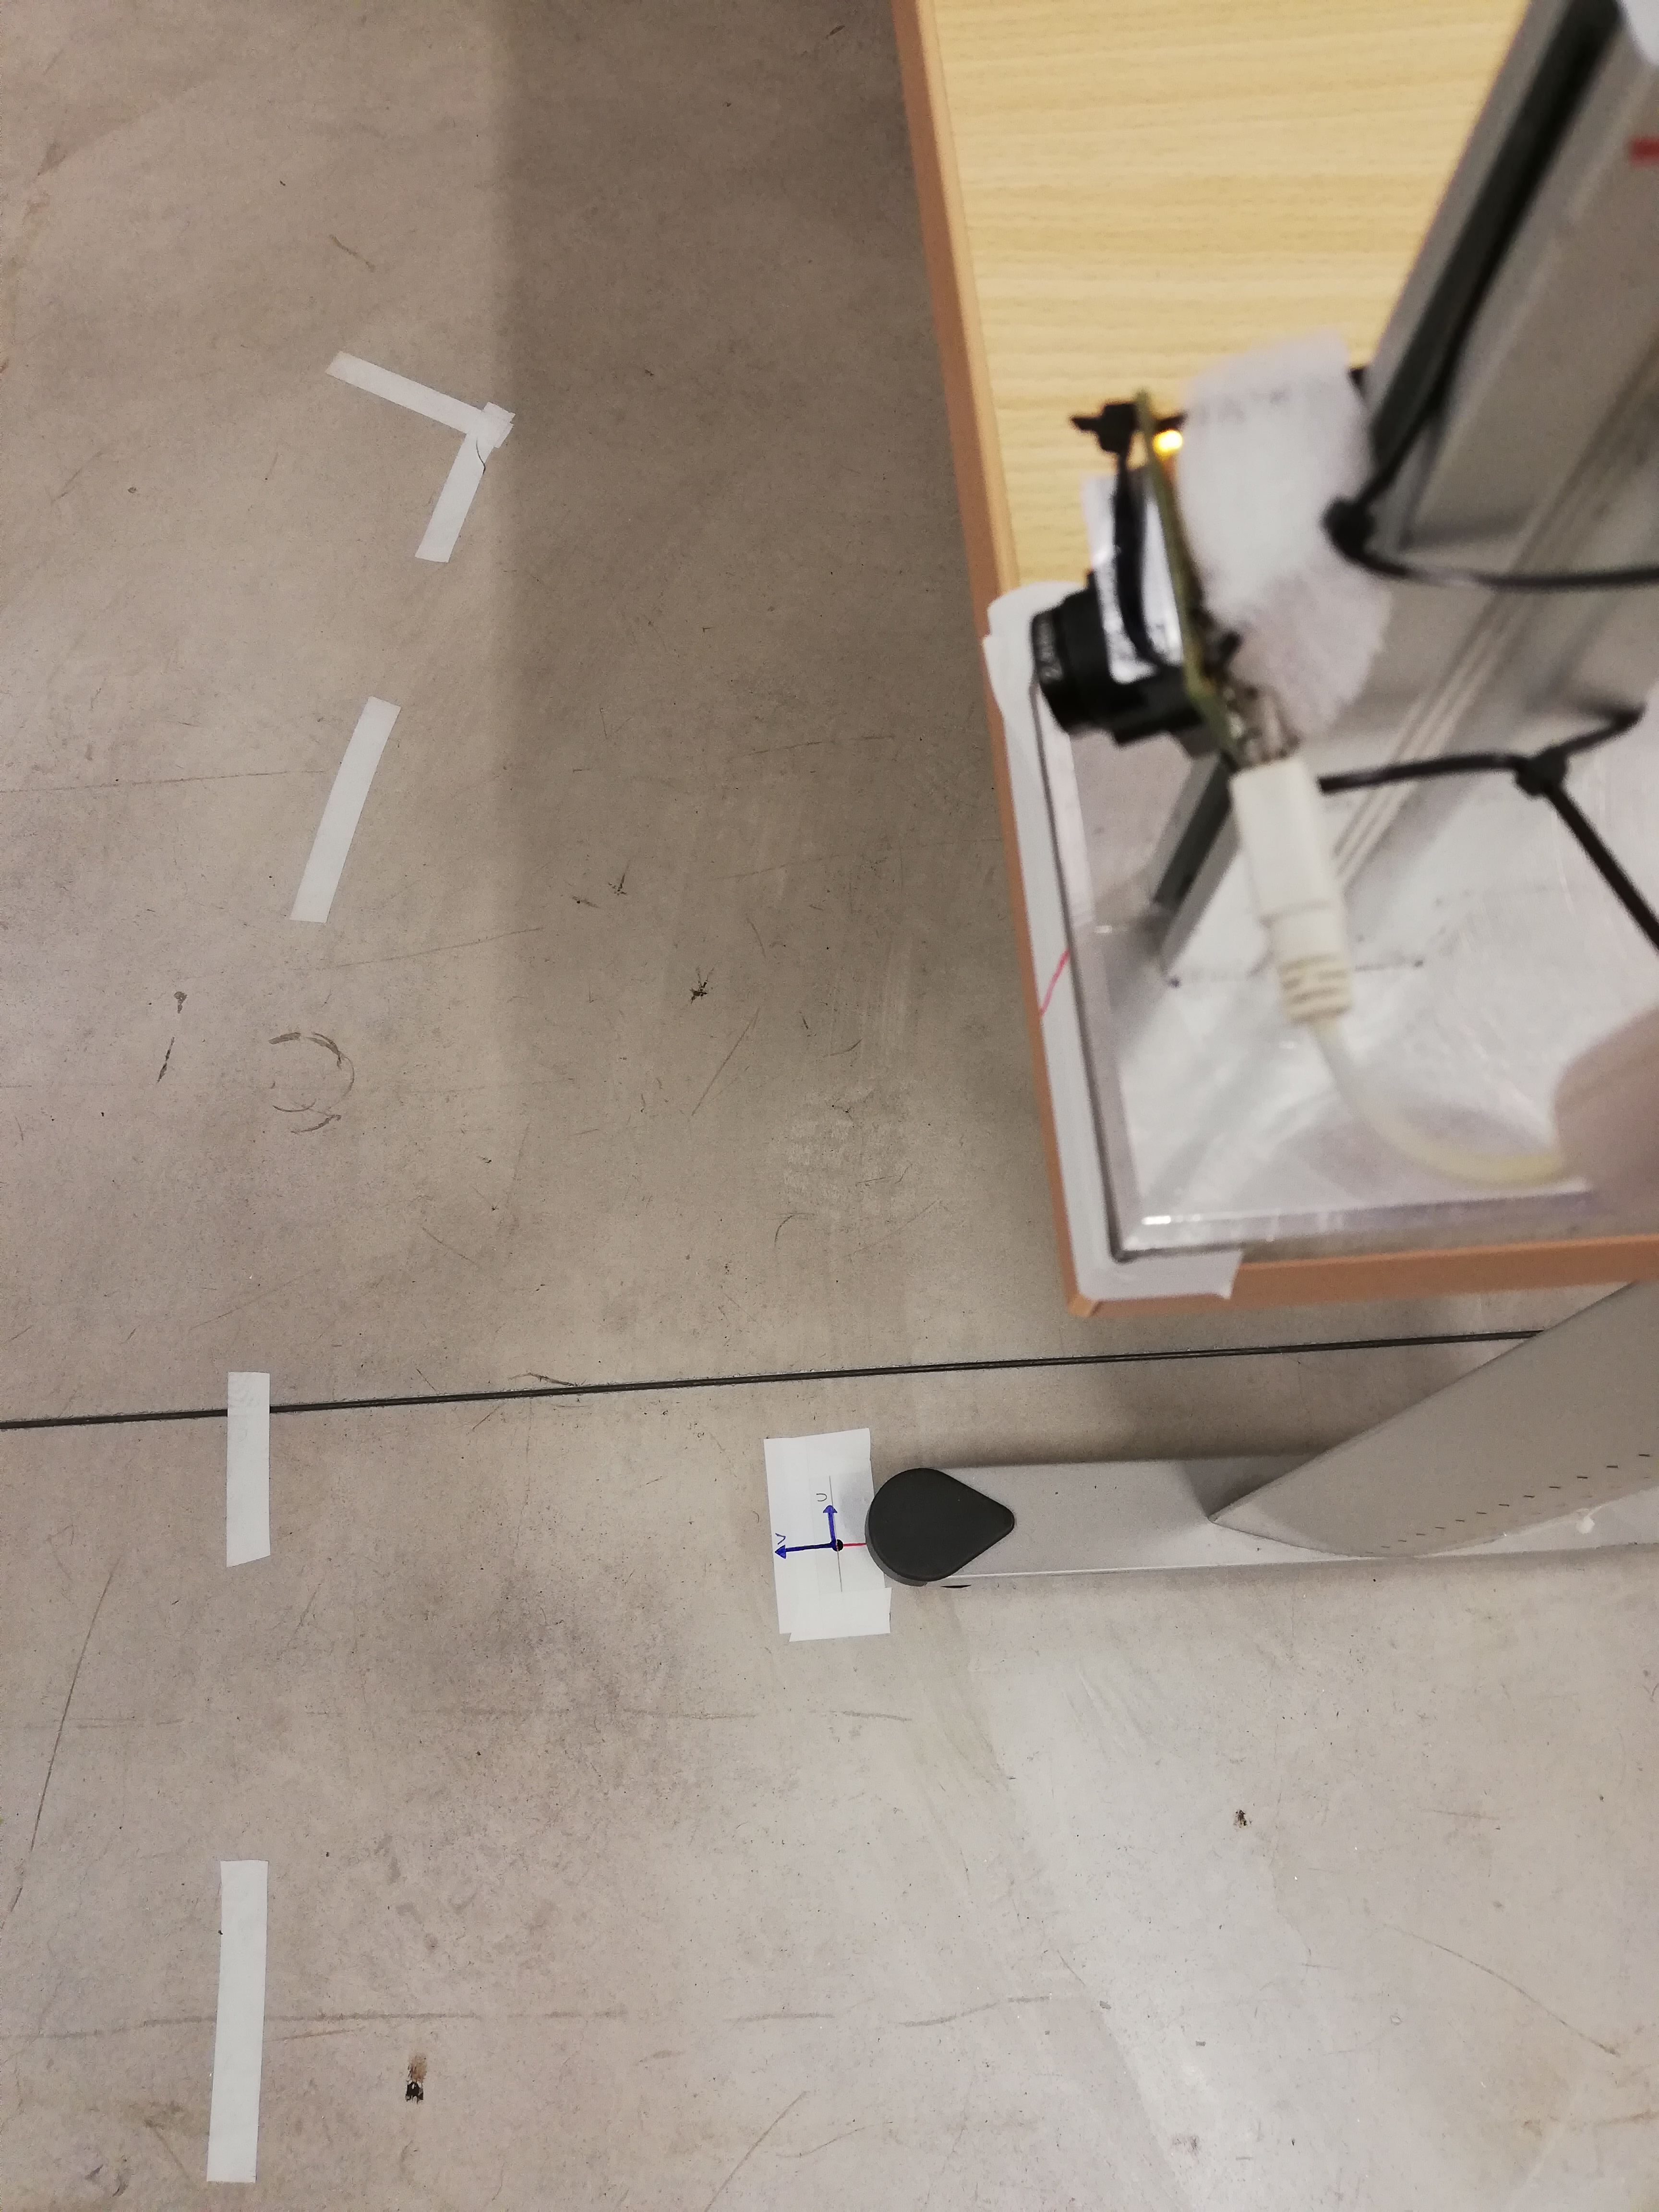
\includegraphics[width=0.8\textwidth]{Immagini/CameraUp.jpg}
	\caption{Frame della camera}
	\label{fig:camera_up}
\end{figure}

\begin{figure}[H]
	\centering
	\includegraphics[width=0.8\textwidth]{Immagini/camera_opposite_pov.jpg}
	\caption{Visione d'insieme dei frames scelti all'interno dell'area di lavoro}
	\label{fig:all_frames}
\end{figure}

\begin{figure}[H]
	\centering
	\includegraphics[width=0.8\textwidth]{Immagini/camera_opposite_pov_2.jpg}
	\caption{rototraslazione del sistema di riferimento della freccia; l'angolo $\Theta$rappresenta la rotazione rispetto al sistema U'V'W' ed è l'inclinazione calcolata precedentemente.}
	\label{fig:rot_frame}
\end{figure}
Le seguenti sono le matrici utilizzate nel codice per rappresentare le rotazioni dei sistemi di riferimento.
\begin{lstlisting}
R_traslation << 1,0,0,0,
				0,1,0,0,
				0,0,1,-h_cam,
				0,0,0,1;

R_rot_cam_inclination  << 1,0,0,0,
					      0,cos(cam_inclination),-sin(cam_inclination),0,
						  0,sin(cam_inclination),cos(cam_inclination),0,
						  0,0,0,1;

R_rot_camera << 1,0,0,0,
				0,cos(M_PI/2),-sin(M_PI/2),0,
				0,sin(M_PI/2),cos(M_PI/2),0,
				0,0,0,1;
\end{lstlisting}
	\chapter{Successive modifiche}
	\section{modificare l'altezza della camera}
Per effettuare modifiche all'altezza della camera è sufficiente modificare il parametro $h_{cam}$ della matrice :
\begin{equation}
	R_{traslazione}\\
	\begin{pmatrix}
	1 & 0 & 0 & 0 \\
	0 & 1 & 0 & 0 \\
	0 & 0 & 1 & h_{cam}\\
	0 & 0 & 0 & 1 \\
	\end{pmatrix}
\end{equation}
Nel caso di modifiche anche rispetto ad altri assi quali U e V sarà sufficiente modificare i valori dei primi due elementi della quarta colonna che rappresentano rispettivamente l'asse U e l'asse V.

\section{modificare l'inclinazione della camera}
Per effettuare eventuali modifiche alla inclinazione della camera, sempre ammesso che il piano Z si voglia uscente dal piano della camera allora sara sufficiente modificare il parametro $\alpha$
\begin{equation}
	R_{rotazione} =
	\begin{pmatrix}
		cos(\dfrac{\pi}{2}+\alpha) & -sin(\dfrac{\pi}{2}+\alpha) & 0 & 0 \\
		sin(\dfrac{\pi}{2}+\alpha) & cos(\dfrac{\pi}{2}+\alpha)& 0 & 0 \\
		0 & 0 & 1 & 0 \\
		0 & 0 & 0 & 1 \\
	\end{pmatrix}
\end{equation}

\section{modificare il terreno su cui si trova il robot}
Nel caso in cui il robot su cui è montata la camera dovvesse essere utilizzato in ambienti diversi da quelli di un laboratorio in cui sono assenti salite, discese o dislivelli allora sarà necessario modificar il piano su cui la freccia giace.
Per fare ciò sarà necessario ricalcolare il piano su cu giace la freccia $ax+by+cz+d=0$ e ricalcolare il fattore di scala
\begin{equation}
	\begin{split}
	s = \dfrac{-d}{aX'+bY'+c}	
	\end{split}
\end{equation}

Si note come, se il robot dovesse viaggiare su un pavimento senza variazioni lungo l'asse U allora il fattore di scala è definito come:
$$
s = \abs{\dfrac{h_{cam}
	}{-sin(\dfrac{\pi}{2}+\alpha)*Y'+ cos(\dfrac{\pi}{2}+\alpha)}}
$$
	\chapter{Indicazioni per l'utilizzo della libreria}
	\begin{lstlisting}
================== SECTION 1: terminator commands=================

Scrivere contemporaneamente su tutti terminali e su tutti quelli che verranno aperti(terminator):
CMD 1:  cd ArrowFinder/devel/; . setup.bash
CMD 2: cd ..

Terminale 1 
caricare il bash da devel (CMD1)
avviare roscore

Terminale 2
caricare il bash da devel (CMD1)
rosrun arrow_finder arrow_finder_node

Terminale 3 (ueye cam)
caricare il bash da devel (CMD1)
cd ~/ArrowFinder/src/ueye_cam/launch
roslaunch debug.launch 

Terminale 4 (throttle)
rosrun topic_tools throttle messages /camera/image_raw 5.0 

================== SECTION 2: deamon =================

Prima di andare sul terminale 4 e necessario, avviare il daemon della camera (solo se non e gia attivo:  esempio:un plug a caldo, da verificare con il programma uEye).
Lo posso runnare da qualsiasi posizione:
sudo /etc/init.d/ueyeusbdrc start (il comando iniziale permetteva di scegliere tra usb e eth: la nostra camera e usb)!
\end{lstlisting}
	
	\begin{thebibliography}{9}
		\bibitem{bib1}
		\emph{Descrizione della camera}
		\url{https://en.ids-imaging.com/store/ui-1221le-rev-2.html}
		
		\bibitem{bib2}
		\emph{Manuale della camera}
		\url{https://en.ids-imaging.com/IDS/datasheet_pdf.php?sku=AB02422}
		
		\bibitem{bib3}
		\emph{Manuale della lente}
		\url{https://www.lensation.de/product/BM2420/}
		
		\bibitem{bib4}
		\emph{Ueye cam e ROS}
		\url{http://wiki.ros.org/ueye}
		
		\bibitem{bib5}
		\emph{HSV vs RGB}
		\url{https://medium.com/neurosapiens/segmentation-and-classification-with-hsv-8f2406c62b39}
		
		\bibitem{bib6}
		\emph{HSV vs RGB}
		\url{https://handmap.github.io/hsv-vs-rgb/}
		%%%%%%%%%%%%%%%%%%%%%%%%%%%%%%%%%%%%%%%%%%%%
		\bibitem{bib7}
		\emph{Camera Projection I}
		\url{http://www.cse.psu.edu/~rtc12/CSE486/lecture12.pdf}
		%%%%%%%%non so dove metterle%%%%%%%%%%%%%%%%%%%
		\bibitem{bib8}
		\emph{Camera Projection II}
		\url{http://www.cse.psu.edu/~rtc12/CSE486/lecture13.pdf}
		
		\bibitem{bib9}
		\emph{Coordinate omogenee}
		\url{http://robotics.unibg.it/teaching/robotics/pdf/14_Geometria3D.pdf}
		
		\bibitem{bib10}
		\emph{Calibrazione camera I}
		\url{http://www.ce.unipr.it/people/medici/geometry/node145.html}
	
		\bibitem{bib11}
		\emph{Calibrazione camera II}
		\url{http://wiki.ros.org/camera_calibration}
		%%%%%%%%%%%%%%%%%%%%%%%%%%%%%%%%%%%%%%%%%%%%%%%%
		\end{thebibliography}

\end{document}
